\documentclass[12pt, letterpaper]{article}
\usepackage{graphicx} % images
\usepackage[a4paper, left=2cm, right=2cm, top=2.5cm, bottom=2.5cm]{geometry}
\usepackage{amssymb}
\usepackage{amsmath}
\usepackage{gensymb}

\title{Analysis H Notes}
\author{Hayden L}
\date{2024-2025}

\begin{document}

\maketitle
\pagebreak

\section{Introduction}
These are my notes for Gunn High School Analysis Honors Course.
\pagebreak

\section{Geometric Approach to Matrices (GAtM)}
\subsection{Groups}\
\textbf{Group}: a set of elements with a binary operation (two inputs, one output)
\begin{enumerate}
    \item \textbf{Identity}: there is an identity element \(I \in G\), \(X \cdot I = I \cdot X = X\)
    \item \textbf{Inverse}: each element \(X\) has an inverse \(X^{-1}\) such that \(X \cdot X^{-1} = X^{-1} \cdot X = X\)
    \item \textbf{Associativity}: \(X \cdot (Y \cdot Z) = (X \cdot Y) \cdot Z\)
    \item \textbf{Closure}: If \(X \in G\) and \(Y \in G\), then \(X \cdot Y \in G\)
\end{enumerate}
\textbf{Order}: the number of elements in a finite group
\begin{itemize}
    \item \textbf{Snap Group} \(S_n\) (\(n\)-post snap group) has an order of \(n!\)
    \item \textbf{Dihedral Group} \(D_n\) (rotation and reflections of a regular \(n\)-gon) has an order of \(2n\)
    \item \textbf{Cyclic Group} \(C_n\) (rotation of a regular \(n\)-gon) has a order of \(n\)
\end{itemize}
\textbf{Period} of an element \(X\): the least possible integer \(n\) such that \(X^n = I\)\\
\textbf{Isomorphic} (Isomorphism of a group): two groups with the same order, inverse, periods, and table\\
\textbf{Generators} of a set are elements that can express \underline{all elements of a group} (also known as the smallest generating set).\\
\textbf{Subgroups}: elements in a group that are closed among themselves..

\subsection{Infinities and Infinite Groups}
\textbf{Countable Infinity}: numbers that can be put in one-to-one correspondence with the set of natural numbers \(\mathbb{N}\)\\
\textbf{Uncountable Infinity}: numbers that cannot be put in one-to-one correspondence with the set of natural numbers \(\mathbb{N}\)\\
\textbf{Cardinality}\footnote{Cardinality refers to the number of elements in a set, while isomorphism refers to the structure. Groups that are isomorphic have the same cardinality, but not all groups with the same cardinality are isomorphic.}: Two infinite sets have the same cardinality if their elements can be put into a one-to-one correspondence with each other.

\centering{\textbf{Number Sets}}
\begin{table}[h]
    \centering
    \begin{tabular}{|c|c|c|}
        \hline
        \textbf{Type of Number}  & \textbf{Definitions} & \textbf{Examples}  \\ \hline
        Natural Numbers \(\mathbb{N}\) & all positive integers from 1 to infinity & 1,2,3,... \\ \hline
        Integers \(\mathbb{Z}\) & a whole number that can be positive, negative, or zero  & ...,-1,0,1,...   \\ \hline
        Rational Numbers \(\mathbb{Q}\) &  numbers that can be expressed as a fraction  & \(\frac{2}{3}, 0.5\)   \\ \hline
        Irrational Numbers \(\mathbb{I}\) & numbers that cannot be expressed as a fraction & \(\sqrt{2}, \pi\)   \\ \hline
        Real Numbers \(\mathbb{R}\)  & the union of both rational and irrational numbers  & N/A  \\ \hline
        Imaginary Numbers & a square root of a negative number  & \(i\)  \\ \hline
        Complex Numbers \(\mathbb{C}\)  & the union of both real and imaginary numbers  & \(1+i\)  \\ \hline
    \end{tabular}
    \caption{Types of Numbers}
    \label{Table 1}
\end{table}
\pagebreak
\raggedright
Since not all infinities are equally big, we can prove that infinite sets have the same cardinality by:
\begin{enumerate}
    \item making a one-to-one correspondence between the sets, or 
    \item if you can prove that \(|A| \geq |B|\) and \(|A| \leq |B|\), then \(|A|=|B|\).\footnote{This means if you find two injective functions, \(f: A\rightarrow B\) and \(g: B\rightarrow A\), then there exists a bijective function \(h: A\rightarrow B\), according to the Cantor-Schroeder-Bernstein Theorem. }
\end{enumerate}
Comparing the set of standards for numbers, we get \[|\mathbb{N}|=|\mathbb{Z}|=|\mathbb{Q}|<|\mathbb{R}|=|\mathbb{C}|\] For example, we can prove that \underline{Natural Numbers and Integers} have the same cardinality (\(|\mathbb{N}|=|\mathbb{Z}|\)) by creating a one-to-one correspondence \[\mathbb{N}\quad\mathbb{Z}\] \[1\Leftrightarrow0\] \[2\Leftrightarrow1\] \[3\Leftrightarrow-1\] \[4\Leftrightarrow2\] \[5\Leftrightarrow-2\] \[...\] thus showing that \(\mathbb{N}\) and \(\mathbb{Z}\) have the same cardinality.
\vspace{1em}\\

We can also find a one-to-one correspondence between \underline{natural numbers and rational numbers} greater than zero.\\
\begin{figure}[h]
    \centering
    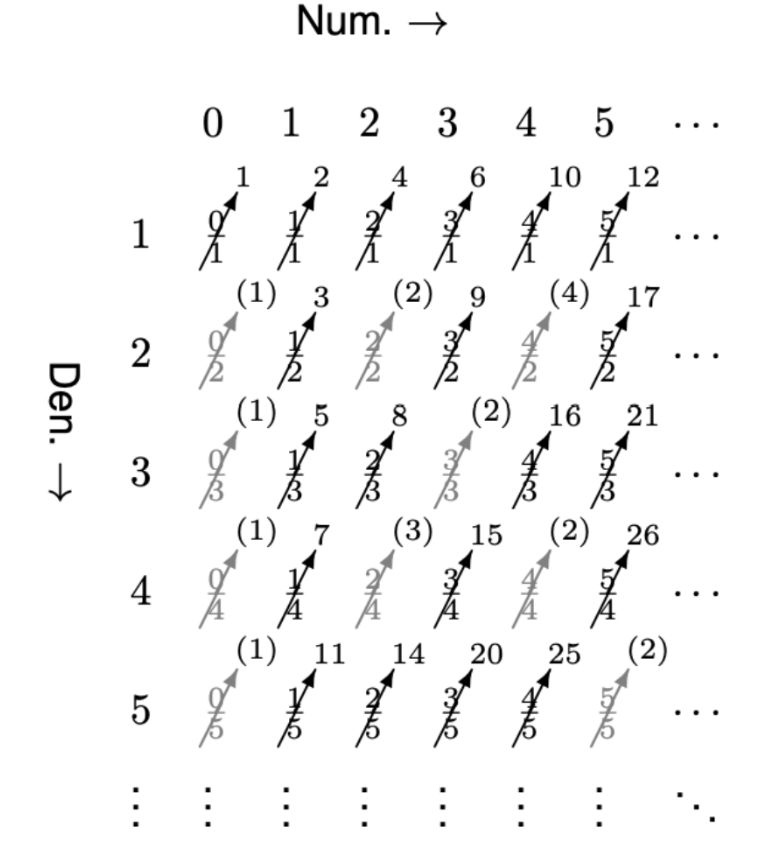
\includegraphics[width=0.45\textwidth]{images/naturalvsrational.png}\\
    \caption{Image 1: \( \mathbb{N} \) vs \( \mathbb{Q}_{\geq 0} \)}
    \label{fig: image1}
\end{figure}
\pagebreak

Now we can compare the infinite sets as listed on GAtM 5.9
\begin{table}[h]
    \centering
    \begin{tabular}{|c|l|c|l|}
        \hline
        & \textbf{Infinite Sets} & \textbf{Group?} & \textbf{Reason} \\ \hline
        a & natural numbers, addition & No & 0 not in group \\ \hline
        b & integers, addition & Yes & \\ \hline
        c & even integers, addition & Yes & \\ \hline
        d & odd integers, addition & No & odd + odd = even \\ \hline
        e & rational numbers, addition & Yes & \\ \hline
        f & real numbers, addition & Yes & \\ \hline
        g & complex numbers, addition & Yes & \\ \hline
        h & integers, multiplication & No & 0 has no identity \\ \hline
        i & integer powers of 2, multiplication & No & \\ \hline
        j & rational numbers, multiplication & No & 0 has no identity \\ \hline
        k & rational numbers excluding 0, multiplication & Yes & \\ \hline
        l & real numbers excluding 0, multiplication & Yes & \\ \hline
        m & complex numbers, multiplication & No & 0 has no identity \\ \hline
        n & rotation by a rational number of degrees & Yes & \\ \hline
        o & rotation by a rational number of radians & Yes & \\ \hline
        p & rotation by an integer number of radians & Yes & \\ \hline
    \end{tabular}
    \caption{Groups of Infinite Sets}
    \label{tab:groups_infinite_sets}
\end{table}\\
We can then see that groups b, c, i, and p are isomorphic to each other, groups e and o are isomorphic to each other, and groups f and g are isomorphic to each other.

\subsection{Geometry of Complex Numbers}
As a refresher of complex number terminology and notation:
\vspace{1em}\\

\textbf{Complex number in rectangular form}: \(z=a+bi\)\\
\textbf{Re(z)}: real part of \(z\), \(Re(z)=a\)\\
\textbf{Im(z)}: imaginary part of \(z\), \(Im(z)=b\)\\
\textbf{Arg(z)}: angle of \(z\) from the positive x-axis\\
\(|\)\textbf{z}\(|\): the length of \(z\), \(|z|=\sqrt{a^2+b^2}\)\\
\textbf{Conjugate of z}: \(\overline{z}=a-bi\)\\
\textbf{cis form}: \(z = |z| \, \text{cis} \, \theta \text{ or } z = r \, \text{cis} \, \theta, \text{where cis} \, \theta = \cos \theta + i \sin \theta\)
\vspace{1em}\\

Now, we can begin with De Moivre's Thereom, where \[(r \, \text{cis} \, \theta)^n = r^n \, \text{cis} \, (n\theta) \text{.}\] 
We can prove De Moivre's Theorem by showing \(r_1( \, \text{cos} \, A+i \, \text{sin} \, A)\cdot r_2( \, \text{cos} \, B+i \, \text{sin} \, B)\).\footnote{see slides}\footnote{Note that \(z\) and \(zi\) are always perpendicular.}
\vspace{1em}\\
\pagebreak

\textbf{\textit{n}-th roots of a complex number}: when finding the \(n\)-th roots of a complex number, you must make sure to find \underline{all} of the solutions. For instance, when finding \(\sqrt[n]{z}\), \[\sqrt[n]{z}\] \[=(r \, \text{cis} \, \theta)^{\frac{1}{n}}\] \[=r^{\frac{1}{n}} \, \text{cis} \, (\frac{\theta}{n}+\frac{2\pi k}{n})\] \[\text{for} \,k = 0,1,2,...,n-1\]
These \(n\) solutions are a result of the Fundamental Theorem of Algebra, which states that any polynomial of degree \(n\) has \(n\)-roots.

\subsection{Mapping the Plane with Matrices}
When mapping a matrices, consider a matrix representing a unit square \(M=
\begin{bmatrix}
0 & 1 & 1 & 0 \\
0 & 0 & 1 & 1
\end{bmatrix}\) and a transformation matrix. The following are a list of transformation matrices.\footnote{The identity, dilation, and some rotations and reflections have a corresponding complex number.} \vspace{1em}\\ 

\textbf{Identity}: \(
\begin{bmatrix} 
1 & 0 \\ 
0 & 1 
\end{bmatrix}\)\vspace{1em}\\

\textbf{Reflection over x-axis}: \(
\begin{bmatrix} 
1 & 0 \\ 
0 & -1 
\end{bmatrix}\)\vspace{1em}\\

\textbf{Reflection over y-axis}: \(
\begin{bmatrix} 
-1 & 0 \\ 
0 & 1 
\end{bmatrix}\)\vspace{1em}\\

\textbf{Reflection over line \textit{y=x}}: \(
\begin{bmatrix} 
0 & 1 \\ 
1 & 0 
\end{bmatrix}\)\vspace{1em}\\

\textbf{Rotation by \(\boldsymbol{\theta}\)}\footnote{Identical to multiplying by \(r \, \text{cis} \, \theta\).}: \(
\begin{bmatrix} 
\text{cos}\,\theta & -\text{sin}\,\theta \\ 
\text{sin}\,\theta & \text{cos}\,\theta 
\end{bmatrix}\)\vspace{1em}\\

\textbf{Stretch by \textit{k} in x-direction}: \(
\begin{bmatrix} 
k & 0 \\ 
0 & 1 
\end{bmatrix}\)\vspace{1em}\\

\textbf{Stretch by \textit{k} in y-direction}: \(
\begin{bmatrix} 
1 & 0 \\ 
0 & k 
\end{bmatrix}\)\vspace{1em}\\

\textbf{Shear\footnote{Shear is a type of linear transformation that distorts the shape of an object such that its points shift parallel to a given axis. Line that were originally parallel remain parallel and area remains the same, but angles between lines and lengths of line segments may change.} by \textit{k} in x-direction}: \(
\begin{bmatrix} 
1 & k \\ 
0 & 1 
\end{bmatrix}\)\vspace{1em}\\

\textbf{Shear by \textit{k} in y-direction}: \(
\begin{bmatrix} 
1 & k \\ 
0 & 1 
\end{bmatrix}\)\vspace{1em}\\

\textbf{Dilation with factor \textit{k}}: \(
\begin{bmatrix} 
k & 0 \\ 
0 & k 
\end{bmatrix}\)\vspace{1em}\\

\textbf{Translation by \(\boldsymbol{<\alpha,\beta>}\)}: \(
\begin{bmatrix} 
1 & 0 & \alpha \\ 
0 & 1 & \beta \\
0 & 0 & 1
\end{bmatrix}
\begin{bmatrix} 
x \\ 
y \\
1
\end{bmatrix}=
\begin{bmatrix}
x+\alpha \\
y+\beta \\
1
\end{bmatrix}\) \vspace{1em}\\

\textbf{Composite of two or more transformations}: When doing two or more transformations, the matrix written first is done second. Consider a rotation by \(90\degree\) and a reflection over the \(y\)-axis. If we were to do the reflection followed by the rotation, we would notate it \[R_{90\degree} \, r_y\text{,}\] while if we were to the rotation first, we would notate it \[r_y \, R_{90\degree}\text{.}\] The former order of transformations is identical to a reflection over the line \(y=-x\), where the latter is identical to a reflection over the line \(y=x\). You can also do a transformation with matrix \(\begin{bmatrix} 
a & b \\
c & d
\end{bmatrix}\) and translation by vector \(<\alpha,\beta>\) by using 3D matrices. Consider doing the transformation first to get \(\begin{bmatrix} 
1 & 0 & \alpha \\ 
0 & 1 & \beta \\
0 & 0 & 1
\end{bmatrix}
\begin{bmatrix} 
a & b & 0 \\ 
c & d & 0 \\
0 & 0 & 1
\end{bmatrix}
=
\begin{bmatrix} 
a & b & \alpha \\ 
c & d & \beta \\
0 & 0 & 1
\end{bmatrix}\).
\vspace{1em}\\

\textbf{Mapping points onto a line}: given a line \(ax+by=0\), we can use a matrix: \(
\begin{bmatrix} 
b & b \\ 
-a & -a 
\end{bmatrix}\) to map the points onto the line. To map the points onto a line \(y=\frac{a}{b}x+c\), we can use a 3D matrix.
\vspace{1em}\\

\textbf{Reflection over the line \(\boldsymbol{\theta=n\degree}\)} (i.e. line with equation \(y=x\,\text{tan}\,\theta)\): \(
\begin{bmatrix} 
\text{cos}2\theta & \text{sin}2\theta \\ 
\text{sin}2\theta & -\text{cos}2\theta 
\end{bmatrix}\).
\vspace{1em}\\
This can be derived from the fact that a composite of two reflections is a rotation, noting that the angle of the rotation is double the angle between the lines of reflection: \[r_{xtan\theta}\cdot r_x=R_{2\theta}\] \[r_{xtan\theta}\cdot r_x\cdot r_x^{-1}=R_{2\theta}\cdot r_x^{-1}\] \[r_{xtan\theta}=R_{2\theta}\cdot r_x^{-1}\] \[r_{xtan\theta}=R_{2\theta}\cdot r_x\]

\pagebreak
\section{Limits}
\subsection{Convergence}\
\textbf{Definition of Convergence:}\footnote{If a sequence does NOT converge, then it diverges.} A sequence \{$a_n$\} is said to converge to a limit $A$ if for any neighborhood of $A$, there can be found a natural number $M$ such that whenever $n\geq M$, \{$a$\} is in the neighborhood of $A$. \vspace{1em}\\
In other words, for any given neighborhood, there is a finite number of terms outside the neighborhood.\vspace{1em}\\
\textbf{Proof for a general $\epsilon$:}\footnote{This is less complicated than the Delta-Epsilon Proof} \[\text{Let } \epsilon > 0 \] \[\text{Given } \lim_{x\to\infty} f(x) = A\footnote{Assume A is a known finite number}\] \[A-\epsilon < f(x) < A+\epsilon\] Then solve for $x$ in terms of $\epsilon$ to prove that: For all natural $n\geq\text{n in terms of } \epsilon$, $f(x)$ is within $\epsilon$ of $A$. Therefore, $\lim_{x\to\infty} f(x) = A$

\subsection{Tests for Convergence and Divergence of Sequences}\
\textbf{Comparison Principle:} The Comparison Principle for sequences can be used to compare a sequence to the terms of a simpler sequence to prove divergence. \vspace{1em}\\
We can use sequences such as \{n\} and \{-n\} as they are both simple and obviously divergent. \vspace{1em}\\

\textbf{Big Theorem:} If a sequence can be proved to be everywhere increasing and bounded above, or everywhere decreasing and bounded below, then it converges. The lowest upper bound, or the highest lower bound, is its limit. \vspace{1em}\\

\textbf{P-Series Test:} For sequences $n^p$ and $p^n$, the following cases diverge\footnote{Other values of p will lead to convergence and is flipped for reciprocals} \[\{n^p\} \text{ where } p>0\] \[\{p^n\} \text{ where } p>1 \text{ or } p\leq-1\footnote{When $p\leq-1$, $p^n$ becomes an alternating sequence that is not practical for the comparison principle}\] \vspace{1em}\\

\textbf{Subsequence Principle:} If $b_n$ is everywhere increasing, $a_n$ increases without bound, and $a_n$ is a subsequence of $b_n$, then $b_n$ increases without bound (is divergent). \vspace{1em}\\

\textbf{Domination Principle:} If two sequences $\{a_n\}$ and $\{c_n\}$ both converge to the same limit L and $\{a_n\}\leq\{b_n\}\leq\{c_n\}$ for all $n$ greater than or equal to some natural number M, then $\{b_n\}$ converges to the same limit L.

\subsection{Series}
\textbf{Series:} \[\sum_{n=1}^{\infty}a_n = a_1+a_2+a_3+a_4+...\] \vspace{1em}\\
\textbf{Sequence of Partial Sums:} \[\{S_1, S_2, S_3, ...\} \text{ where } S_1 = a_1, S_2 = a_1+a_2, ...\] \vspace{1em}\\
A few important sequences to take note of are $\{\frac{1}{n^2}\}$ and $\{\frac{1}{n}\}$. \footnote{Also known as the harmonic series} \[\sum_{n=1}^{\infty}\frac{1}{n^2} = 1+\frac{1}{4}+\frac{1}{9}+\frac{1}{16}+...+\frac{1}{n^2}=\frac{\pi^2}{6} \text{; Converges}\] \[\sum_{n=1}^{\infty}\frac{1}{n} = 1+\frac{1}{2}+\frac{1}{3}+\frac{1}{4}+...+\frac{1}{n}=\infty \text{ or DNE; Diverges}\] \vspace{1em}\\

\subsection{Tests for Convergence and Divergence of Series}
\textbf{Geometric Series Test:} Given the geometric series $S = a+ar+ar^2+ar+3+...$, the geometric series converges to $\frac{a}{1-r}$ if $|r|<1$, otherwise it diverges. \[\text{If } |r|<1\implies\sum_{n=1}^{\infty}a(r)^{n-1} = \frac{a}{1-r}\] \vspace{1em}\\
\textbf{nth Term Test:} If the sequence $\{a_n\}$ does not converge to 0, then the series $\sum_{n=1}^{\infty}a_n$ diverges. Be careful in using this test as this test can NOT prove convergence of a series. \[\lim_{n\rightarrow\infty}a_n\neq0 \implies \sum_{n=1}^{\infty}a_n=\infty \text{ or DNE}\] \vspace{1em}\\
\textbf{P-series Test:} Since we know from sequences that $\{n^p\}$ diverges for all $p>0$ and that $\{\frac{1}{n^p}\}$ converges for all $p\geq0$, the series of $\frac{1}{n^p}$ will converge if and only if $p>1$. \footnote{Note that $\sum_{n=1}^{\infty}\frac{1}{p^n}$ is just a geometric series and thus can be found through the Geometric Series Test.}\[p\leq1\implies\sum_{n=1}^{\infty}\frac{1}{n^p}=\infty\] \vspace{1em}\\
\textbf{Comparison Test\footnote{Not to be confused with the sequence test, comparison principle.}:} If $\{a_n\}$ and $\{b_n\}$ are two sequences such that $0<a_n\leq b_n$ for all natural numbers $n$, then:
\begin{enumerate}
    \item If $\sum_{n=1}^{\infty} a_n$ diverges, then $\sum_{n=1}^{\infty} b_n$ also diverges.
    \item If $\sum_{n=1}^{\infty} b_n$ converges, then $\sum_{n=1}^{\infty} a_n$ also converges.
\end{enumerate}
Take note that you cannot prove that $\sum_{n=1}^{\infty} a_n$ diverges or that $\sum_{n=1}^{\infty} b_n$ converges. \vspace{1em}\\
\textbf{Ratio Test:} For a sequence $\{a_n\}$, consider $b$ in: \[\lim_{n\rightarrow\infty}|\frac{a_{n+1}}{a_n}=b\]
\begin{enumerate}
    \item If $0\leq b<1$, then the series converges.
    \item If $b>1$, then the series diverges.
    \item If $b=1$, then this test is inconclusive and another test must be used to prove its convergence or divergence.
\end{enumerate} 
\textbf{Alternating Series Test:} A series $\sum_{n=1}^{\infty} a_n$ will converge if and only if:
\begin{enumerate}
    \item The sequence is strictly alternating in signs,
    \item Everywhere decreasing in absolute value (approaches 0)
    \item And the sequence converges to 0.
\end{enumerate}

\section{Calculus}
\subsection{Integral: Area Under Curve}
\textbf{Sum of Important Sums:\footnote{These will be given on the test and do not need to be memorized.}} \[1+2+3+4+...+n = \frac{n(n+1)}{2}\] \[1^2+2^2+3^2+4^2+...+n^2=\frac{n(n+1)(2n+1)}{6}\] \[1^3+2^3+3^3+4^3+...+n^3=(\frac{n(n+1)}{2})^2\]
\textbf{Definite Integral:} The definite integral is the area under the curve. One way to find the definite integral is by considering rectangles with a width of $\frac{1}{n}$. Consider for example $f(x)=2x$. To find the definite integral over the interval $[0,2]$ \[\frac{1}{n}\sum_{k=1}^{2n}[2(\frac{k}{n})]=A\] Here, $\frac{1}{n}$ is the width of the rectangles, $2n$ is the number of rectangles, and $\frac{k}{n}$ is plugged into $x$. After simplifying using sum equations, find the limit as $n$ approaches $\infty$ to find the indefinite integral \[\lim_{n\rightarrow\infty}[A]\] When finding the definite integral over an interval $[1,2]$, add the starting x value to $\frac{k}{n}$: \[\frac{1}{n}\sum_{k=1}^{n}[2(\frac{k}{n}+1)]\] and solve for the limit as $n$ approaches $\infty$. \vspace{1em}\\
\textbf{Trapezoid Rule:} To approximate the definite integral, you can use the trapezoid rule, where given $y=f(x)$, \[A=\frac{h}{2}(f(a)+2f(a+h)+2f(a+2h)+...+2f(a+(n-1)h)+f(a+nh))\]

\subsection{AROC vs IROC}
\textbf{Average Rate of Change:} Calculated as if there is a straight line between points $(a,f(a))$ and $(b, f(b))$. Over the interval $[a,b]$, the average rate of change would be \[\frac{f(b)-f(a)}{b-a}\]
\textbf{Instantaneous Rate of Change:} Also known as the derivative. This can be \textit{approximated} by using the AROC of two points that are very close together. \[f'(x)=\frac{dy}{dx}\]

\subsection{Limits and Discontinuities}
\textbf{Limits:} A limit exists at $x\rightarrow c$ if and only if \[\lim_{x\rightarrow c^+}f(x)=\lim_{x\rightarrow c^-}f(x)\] and the limit is a finite, non-infinite number. \vspace{1em}\\
\textbf{Continuity:} A function is continuous at point $x=c$ if and only if \[\lim_{x\rightarrow c^+}f(x)=\lim_{x\rightarrow c^-}f(x)=f(c)\]
\begin{enumerate}
    \item $\lim_{x\rightarrow c}f(x)$ exists
    \item $f(c)$ exists
    \item $\lim_{x\rightarrow c}f(x)=f(c)$
\end{enumerate}
\textbf{Discontinuities:}
\begin{enumerate}
    \item Removable discontinuity (hole): The limit exists but is not continuous.
    \item Jump discontinuity: $\lim_{x\rightarrow c^+}f(x)$ and $\lim_{x\rightarrow c^-}f(x)$ exist but $\lim_{x\rightarrow c}f(x)$ does not exist.
    \item Infinite discontinuity (vertical asymptote): both one-sided limits approach infinity, and thus do not exist (DNE). Limit algebraically is $\frac{k}{0}$.
\end{enumerate}
\textbf{Definition of a Limit:} A function $f(x)$ is said to approach a limit $L$ as $x\rightarrow c$ if and only if for any positive $\epsilon$ there exists a positive number $\delta$ such that whenever $x$ is within $\delta$ of $c$, but $x\neq c$, $f(x)$ is within $\epsilon$ of $L$. \[\lim_{x\rightarrow c}f(x)=L \text{ iff } \forall\epsilon>0, \exists\delta>0: 0<|x-c|<\delta\implies|f(x)-L|<\epsilon\]
\textbf{Delta-Epsilon Proof:} Start with epsilon proof: \[L-\epsilon<f(x)<L+\epsilon\] and express $x$ in terms of $\epsilon$. Find $\delta_L$ and $\delta_R$ and set $\delta$ to be the smaller of the two. Finally, write a conclusion statement and plug in values as necessary: \[\text{Let } \epsilon>0, \text{for any }x\text{ within }\delta=\_ \text{ of } c, f(x)\text{ is within } \epsilon \text{ of }L\]
\textbf{Limit Properties:} 
\begin{enumerate}
    \item The limit of a produce equals the product of the limits. \[\lim_{x\rightarrow c}(f(x)\times g(x))=\lim_{x\rightarrow c}(f)\times\lim_{x\rightarrow c}g(x)\]
    \item The limit of a sum equals the sum of the limits. \[\lim_{x\rightarrow c}(f(x)+ g(x))=\lim_{x\rightarrow c}(f)+\lim_{x\rightarrow c}g(x)\]
    \item The limit of a quotient equals the quotient of the limits. \[\lim_{x\rightarrow c}\frac{f(x)}{g(x)}=\frac{\lim_{x\rightarrow c}(f)}{\lim_{x\rightarrow c}g(x)}\]
    \item The limit of a constant times a function equals the constant time the limit. \[\lim_{x\rightarrow c}Cf(x)=C\lim_{x\rightarrow c}(f)\]
    \item The limit of the constant is that constant. \[\lim_{x\rightarrow c}C=C\]
    \item The limit of the identity function is "c". \[\lim_{x\rightarrow c}x=c\]
    \item The limit of a composite is the limit of the inside function with respect to the outside function. \[\lim_{x\rightarrow c}f(g(x))=f(\lim_{x\rightarrow c}g(x))\]
\end{enumerate}
\textbf{Intermediate Value Theorem (IVT):} Given that $f(x)$ is continuous for all $x$ in the interval $[a,b]$, if $y$ is a value between $f(a)$ and $f(b)$, then there is a number $x=c$ in $[a,b]$ for which $f(c)=y$.

\subsection{Derivatives}
\textbf{Formal Definition of the Derivative at a Point (FDoDaP):} \[f'(c)=\lim_{x\rightarrow c}\frac{f(x)-f(c)}{x-c}\]
\textbf{Formal Definition of the Derivative (FDoD):} \[f'(x)=\lim_{h\rightarrow 0}\frac{f(x+h)-f(x)}{h}\]
\textbf{Power Rule:} \[f(x)=x^n \implies f'(x)=nx^{n-1}\]
\textbf{Chain Rule:} \[h(x)=f(g(x)) \implies h'(x)=f'(g(x))g'(x)\] \[\frac{dy}{dx}=\frac{dy}{du}\times\frac{du}{dx}\]
\textbf{Trigonometric Functions:} \[f(x)=\sin(x) \implies f'(x)=\cos(x)\] \[f(x)=\cos(x) \implies f'(x)=-\sin(x)\] \[f(x)=\tan(x) \implies f'(x)=\sec^2(x)\] \[f(x)=\cot(x) \implies f'(x)=-\csc^2(x)\] \[f(x)=\sec(x) \implies f'(x)=\sec(x)\tan(x)\] \[f(x)=\csc(x) \implies f'(x)=- \csc(x)\cot(x)\]

\subsection{Particle Motion}
\textbf{Relation of Derivatives:} Given that $p(t)$ is the position of the particle, $p'(t)=v'(t)$ is the velocity and $s''(t)=v'(t)=a(t)$ is acceleration. Note that the speed of a particle is $|v(t)|$ and the particle is speeding up if $v(t)$ and $a(t)$ have the same sign. 

\subsection{Sinusoids}
\textbf{Sinusoids:} Amplitude is $A$, Period is $\frac{2\pi}{B}$, Phase shift is $C$ (positive to left)\footnote{also remember that $\sin(0)=0$ and $\cos(0)=1$}, and vertical shift is $D$ (midline is $y=D$) \[y=A\sin(B(x+C))+D\]

\subsection{Antiderivatives}
\textbf{Indefinite Integral:} $g(x)$ is the antiderivative of f(x) if and only if $g'(x)=f(x)$. \[\int f(x)dx = g(x)+c\footnote{Make sure to not forget the +c}\]

\subsection{Fundamental Theorem of Calculus}
\[\int_{a}^{b}f'(t)dt=f(b)-f(a)\]
\end{document}